\section{The Symbol Class}
In CUP each symbol in the stack is an object of class Symbol (\code{cup/java_cup/runtime/Symbol.java}).
It contains the following information:
\begin{itemize}
    \item
    a number uniquely identifying the symbol (\code{public int sym});
    \item
    the state in which the parse is (\code{public int parse_state});
    \item
    two integers that are used to pass the line and column numbers from the scanner to the parser (\code{public int left}, \code{public int right});
    \item
    an object of class Object to handle semantics (\code{public Object value}).
\end{itemize}

\subsection{Passing Semantic Values to the Parser}
Example: scanner.jflex

Symbol constructors:
\begin{itemize}
    \item
    \code{public Symbol(int sym_id)};
    \item
    \code{public Symbol(int sym_id, int left, int right)};
    \item
    \code{public Symbol(int sym_id, Object o)};
    \item
    \code{public Symbol(int sym_id, int left, int right, Object o)}
\end{itemize}
Symbol and semantic values:
\begin{lstlisting}
[a-zA-Z][a-zA-Z0-9]* {return new Symbol(sym_id, new String(yytext()));}
\end{lstlisting}
Symbol, line number, column number, and semantic value:
\begin{lstlisting}
%{
    private Symbol symbol(int type, Object value) {
        return new Symbol(type, yyline, yycolumn, value);
    }
%}
\end{lstlisting}

\begin{lstlisting}
[a-zA-Z][a-zA-Z0-9]* {return new Symbol(sym_id, new String(yytext()));}
\end{lstlisting}
or equivalently:
\begin{lstlisting}
[a-zA-Z][a-zA-Z0-9]* {return new Symbol(sym_id, yyline, yycolumn, new String(yytext()));}
\end{lstlisting}

\section{Specifying Nodes Types}
CUP must know the type of the semantic value of each symbol; it uses the following definition of terminals and non-terminals:
\begin{itemize}
    \item
    \code{terminal <Object> <list_of_terminals>;}
    \item
    \code{non terminal <Object> <list_of_non-terminals>;}
\end{itemize}
\code{<Object>} is the class of the object associated to a given symbol.

Example:
\begin{itemize}
    \item
    \code{terminal String ID;} an object of class String will be associated to \code{ID};
    \item
    \code{terminal Integer NUM;}
    \item
    \code{non terminal MyObject var;} will have something like this:
    \begin{lstlisting}
class MyObject {
    public String var_name;
    public String var_type;
}
    \end{lstlisting}
\end{itemize}

\section{Using Semantic Values}
Given a set of productions:
\begin{lstlisting}
E ::= E PLUS T
    | E MINUS T
\end{lstlisting}
One can refer to the semantic value of each symbol by adding labels to the symbol of interest.
A label is constituted by the ``\code{:}'' character, followed by a name.
\begin{lstlisting}
E ::= E:m1 PLUS T:m2
    | E:m1 MINUS T:m2
\end{lstlisting}
Within each production, the labels can be normally used as objects of the class specified in the definition of terminals and non-terminals.
\begin{lstlisting}
E ::= E:m1 PLUS T:m2 {: System.out.println(m1 + " + " + m2); :}
    | E:m1 MINUS T:m2 {: System.out.println(m1 + " - " + m2); :}
\end{lstlisting}

\section{Action and \code{RESULT}}
An action can be associated to each production (\code{\{:/*java code*/:\}}) and is executed every time the corresponding production is reduced.
The action updates the semantic values of each symbol.
For each production, the result object (of class Object) is defined.

\code{RESULT} represents the result of the semantic rules contained in the action and is therefore associated to the symbol in the left hand side of the production.

\subsection{Calculating Synthesized Attributes}
Given the algebraic expression grammar, the following rules assigns to the symbol ``\code{E}'' the sum or the subtraction of the values of the addends/subtrahends.
\begin{lstlisting}[frame=single]
non terminal Integer E;

E ::= E:m1 PLUS T:m2 {:
        RESULT = new Integer(m1.intValue() + m2.intValue());
    :}
    | E:m1 MINUS T:m2 {:
        RESULT = new Integer(m1.intValue() - m2.intValue());
    :}
\end{lstlisting}
Note that \code{RESULT} must be assigned n object of class Integer (\code{new Integer()}); mathematical operators work on numbers, not objects (\code{m1.intValue()}).

It is possible to propagate more than one semantic value through \code{RESULT}.

Example:
\begin{lstlisting}[frame=single]
terminal TO, TC;
terminal String Identifier;
terminal Integer Args;

non terminal Object[] func;
non terminal goal;

goal ::= func:a {:
    System.out.println("Function name: " + a[0] + ", number of parameters: " + a[1]);
:};

func ::= Identifier:a TO Args:b TC {:
    RESULT = new Object[2];
    RESULT[0] = new String(a);
    RESULT[1] = new Integer(b);
:};
\end{lstlisting}
Alternatively, one can write a class that contains all the required information.

Example:
\begin{lstlisting}[frame=single]
action code {:
    class MyFunc {
        public String id;
        public Integer args;
        MyFunc(String id, String args) {
            this.id = id;
            this.args = args;
        }
    }
:}

non terminal MyFunc func;

goal ::= func:a {:
    System.out.println("Function name: " + a.id + ", number of parameters: " + a.args);
:};

func ::= Identifier:a TO Args:b TC {:
    RESULT = new MyFunc(a, b);
:};
\end{lstlisting}

\section{Parser Debugging}
A series of options are available in CUP to visualize the parser's internal structures:
\begin{itemize}
    \item
    \code{-dump_grammar} prints the list of terminals, non-terminals, and productions;
    \item
    \code{-dump_states} prints the states graph;
    \item
    \code{-dump_table} prints the action table and the reduce table;
    \item
    \code{-dump} prints all the information.
\end{itemize}
The parser can be executed in debug mode (all the actions performed to analyze the input sequence are printed).

Example:

Normal mode:
\begin{lstlisting}
                        Yylex l = new Yylex(new FileReader(file));
                        parser p = new parser(l);
                        Object result = p.parse();
\end{lstlisting}

$$
\Downarrow
$$

Debug mode:
\begin{lstlisting}
                        Yylex l = new Yylex(new FileReader(file));
                        parser p = new parser(l);
                        Object result = p.debug_parse();
\end{lstlisting}

\section{Inherited Attributes}
Inherited attributes are useful to express the dependency of a production on its context.

Example:
\begin{lstlisting}
a,b: int;
\end{lstlisting}
\begin{align*}
& D \to L \, ':' \, T \, ';' \\
& L \to L_1 \, ',' \, id \\
& L \to id \\
& T \to 'integer'
\end{align*}
\begin{lstlisting}
L.type = T.type
L1.type = L.type; new_var(id.name, L.type)
new_val(id.name, L.type)
T.type = type_int
\end{lstlisting}

\section{L-Attribute Grammar}
The order in which attributes are evaluated depends on the order in which the parse tree is created ir visited.
Usually, parser follows the same order of the depth-first visit algorithm.\footnote{\url{http://en.wikipedia.org/wiki/Depth-first_search}}

An L-Attribute grammar is defined as a grammar whose attributes values can be calculated by means of a depth-first visit of the parse tree.
In these grammars, information propagates from left to right (within the parse tree).
In the previous example, the grammar is not an L-Attribute grammar (information propagates from right to left); CUP manages only L-Attributes grammar.

Example:
\begin{lstlisting}
int a, b;
\end{lstlisting}
\begin{align*}
& D \to T \, L \, ';' \\
& L \to L_1 \, ';' \, id \\
& L \to id \\
& T \to 'int'
\end{align*}
\begin{lstlisting}
L.type = T.type
L1.type = L.type; new_var(id.name, L.type)
new_val(id.name, L.type)
T.type = type_int
\end{lstlisting}

\subsection{Calculating Inherited Attributes}
In a bottom-up parser, memory is not allocated in the semantic stack until the corresponding symbol is recognized.
This is a troublesome for handling inherited attributes.
If the grammar is an L-Attribute one, and the semantic rules for inherited attributes are copy-rules, the issue can be tackled in a relatively simple way.
If rules are more complex than this, it is possible to use \emph{markers} (non-terminals that are expanded with $\varepsilon$ symbol).

Example: a production with a copy-rule.
\begin{align*}
& D \to T \, lid \, S \\
& lid = ID
\end{align*}
\begin{lstlisting}
lid.type = T.type
var(ID.name, lid.type)
\end{lstlisting}
Stack before \code{lid} is reduced:
%\begin{figure}[H]
%    \centerline{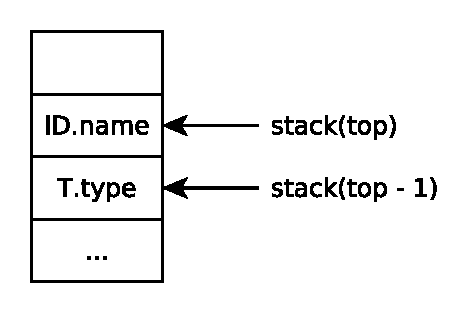
\includegraphics[width=0.4\textwidth]{img/33.pdf}}
%\end{figure}

\subsubsection{Calculating Inherited Attributes by means of Markers}

\section{Intermediate Actions}

\section{Transforming the Grammar}

\section{Handling Semantic Errors}